        \subsection{dither}
	\begin{frame}\frametitle{sampling and quantization}\framesubtitle{requantization and dither: introduction 1/2}
        \begin{columns}
            \column{.5\textwidth}
		\begin{itemize}
			\item	previous assumption: \textbf{quantization error is white noise} (rect)
				\pause
				\begin{itemize}
					\item[$\rightarrow$]	\textbf{no correlation} between signal and quantization error
				\end{itemize}
                \smallskip
			\visible<2->{
			\item	\textbf{not true for}
				\begin{itemize}
					\item	low signal level
					\item	low signal frequency
				\end{itemize}
			}
            \visible<3->{
                \smallskip
             \item	\textbf{solution}:
				\begin{itemize}
					\item	 \textbf{add noise before quantization: dither}
				\end{itemize}
                }
		\end{itemize}
        \column{0.5\textwidth}
			\visible<2->{
      	\begin{figure}
				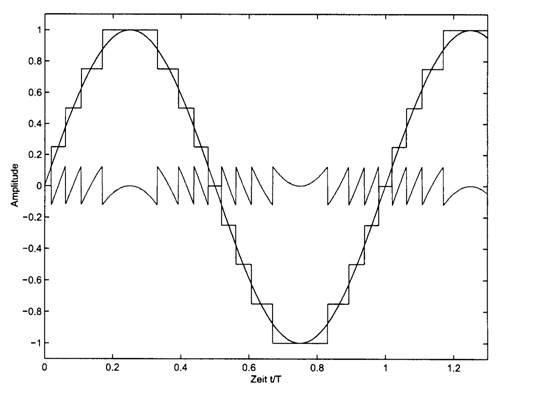
\includegraphics[scale=.45]{Graph/quant+quanterror}
		\end{figure}
        }
    \end{columns}
	\end{frame}	
	\begin{frame}\frametitle{sampling and quantization}\framesubtitle{requantization and dither: introduction 2/2}
		\vspace{-5mm}
        \begin{figure}
			\centering
				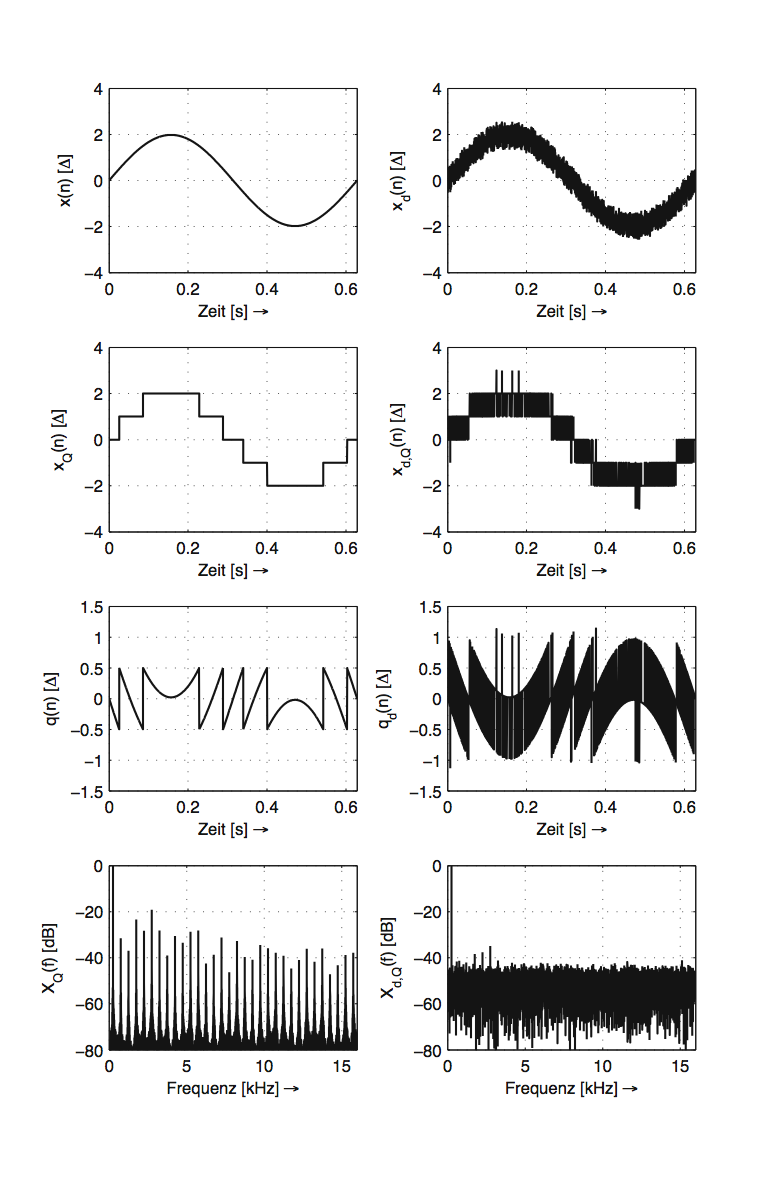
\includegraphics[scale=0.4]{Graph/3stepquantdither.png}
		\end{figure}
	\end{frame}	
	\begin{frame}\frametitle{sampling and quantization}\framesubtitle{requantization and dither: process}
		\begin{figure}
			\centering
				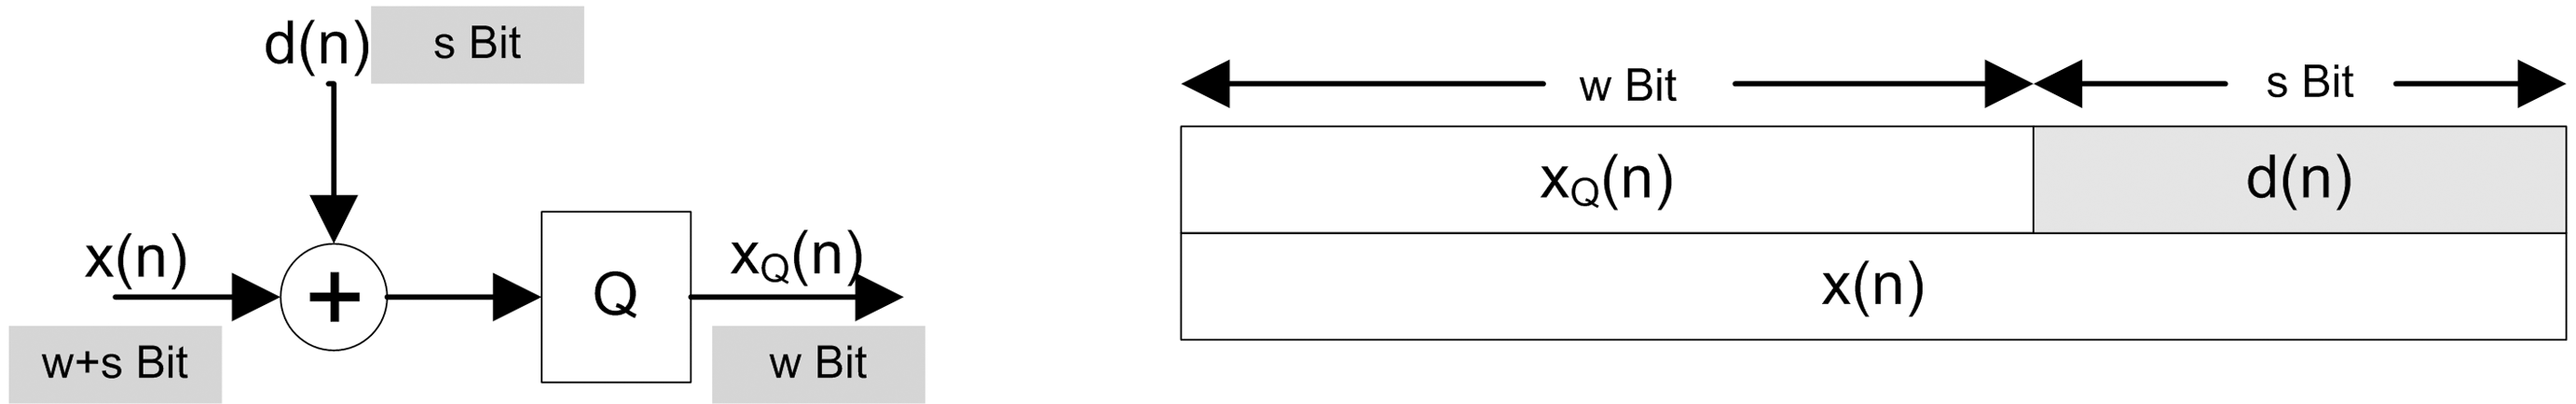
\includegraphics[scale=0.9]{Graph/quantisierung_mit_dither.png}
		\end{figure}
	\end{frame}	
	\begin{frame}\frametitle{sampling and quantization}\framesubtitle{requantization and dither: simple example}
		input signal: DC at $1.3\cdot\Delta$
        \bigskip
		\begin{itemize}
			\item	\textbf{w/o dither}: 
				\begin{itemize}
					\item	output value: $\Delta$
					\item	\textit{quantization error constant}: $.3\cdot\Delta$
				\end{itemize}
			\pause
            \bigskip
			\item	\textbf{w/ dither}: 
				\begin{itemize}
					\item	signal is most frequently quantized to $\Delta$, but sometimes to $2\cdot\Delta$
					\item	\textit{average} output value: $1.3\cdot\Delta$!
                    \item   \textit{quantization error varying} between $0.3\cdot\Delta$ and $0.7\cdot\Delta$
				\end{itemize}
		\end{itemize}
	\end{frame}	
	\begin{frame}\frametitle{sampling and quantization}\framesubtitle{requantization and dither: properties}
		\begin{figure}
			\centering
				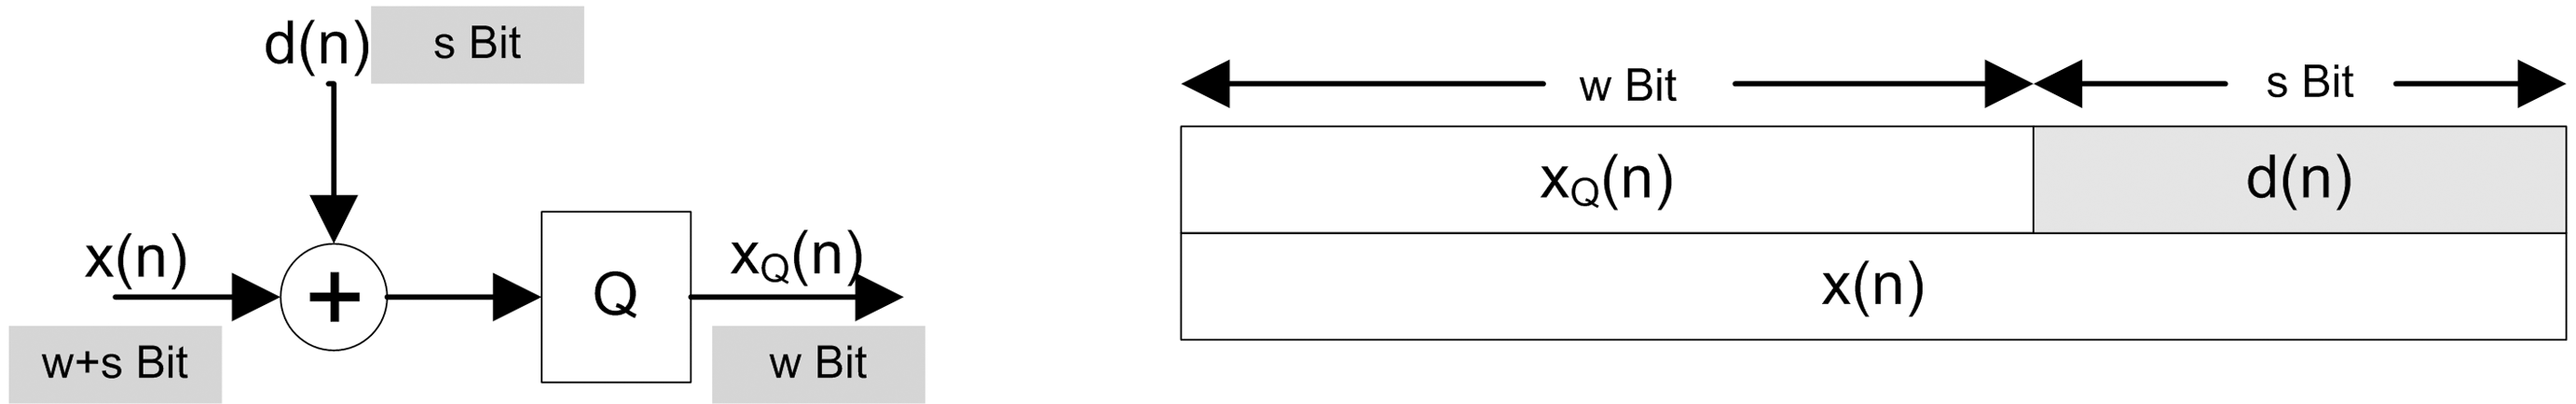
\includegraphics[scale=0.9]{Graph/quantisierung_mit_dither.png}
		\end{figure}
        \pause
        \begin{itemize}
            \item   dither: $2^s$ possible possible numbers
            \pause
            \item   in case of \textit{uniform} dist  $\rightarrow$
            \begin{equation*}
                 p_d(d_n) = \left\lbrace \begin{array}{ll}
                    2^{-s} & -2^{s-1}\leq n \leq 2^{s-1}-1\\
                    0 & \text{else}.
                \end{array}\right.
            \end{equation*}
            \pause
            \item   output
            \begin{equation*}
                x_Q(X + d_n) = \Delta\left\lfloor \frac{X + d_n}{\Delta} + 0.5 \right\rfloor
            \end{equation*}
        \end{itemize}
	\end{frame}	
	\begin{frame}\frametitle{sampling and quantization}\framesubtitle{requantization and dither: rectangular dither}
        \vspace{-5mm}
        dither with rect pdf, $-\nicefrac{\Delta}{2}\ldots \nicefrac{\Delta}{2}$, not quantized
        \begin{itemize}
            \item   $x = 0 \cdot \Delta$ \pause $\rightarrow \bar{x_Q} =0$,\\ $\sigma_R(x) = 0$
            \pause
            \item   $x = 0.1 \cdot \Delta$ \pause $\rightarrow \bar{x_Q} = 0.1 $,\\ $\sigma_R(x) = \sqrt{(-0.1)^2\cdot0.9 + (0.9)^2\cdot0.1} = 0.3$ 
            \pause
            \item   $x = 0.3 \cdot \Delta$ \pause $\rightarrow \bar{x_Q} = 0.3 $,\\ $\sigma_R(x) = \sqrt{(-0.3)^2\cdot0.7 + (0.7)^2\cdot0.3} = 0.46$ 
            \pause
            \item   $x = 0.5 \cdot \Delta$ \pause $\rightarrow \bar{x_Q} = 0.5 $,\\ $\sigma_R(x) = \sqrt{(-0.5)^2\cdot0.5 + (0.5)^2\cdot0.5} = 0.5$ 
            \pause
            \item   $x = 0.7 \cdot \Delta$ \pause $\rightarrow \bar{x_Q} = 0.7 $,\\ $\sigma_R(x) = \sqrt{(-0.7)^2\cdot0.3 + (0.3)^2\cdot0.7} = 0.46$ 
            \pause
            \item   $x = 0.9 \cdot \Delta$ \pause $\rightarrow \bar{x_Q} = 0.9 $,\\ $\sigma_R(x) = \sqrt{(-0.9)^2\cdot0.1 + (0.1)^2\cdot0.9} = 0.3$ 
            \pause
            \item   $x = 1 \cdot \Delta$ \pause $\rightarrow \bar{x_Q} =0$,\\ $\sigma_R(x) = 0$
        \end{itemize}
	\end{frame}	
	\begin{frame}\frametitle{sampling and quantization}\framesubtitle{requantization and dither: triangular dither}
        \vspace{-5mm}
        dither with tri pdf, $-{\Delta}\ldots {\Delta}$, not quantized
        \begin{itemize}
            \item   $x = 0 \cdot \Delta$ \pause $\rightarrow \bar{x_Q} =0$,\\ $\sigma_R(x) = 0.5$
            \pause
            \item   $x = 0.1 \cdot \Delta$ \pause $\rightarrow \bar{x_Q} = 0.1 $,\\ $\sigma_R(x) = 0.5$ 
            \pause
            \item   $x = 0.3 \cdot \Delta$ \pause $\rightarrow \bar{x_Q} = 0.3 $,\\ $\sigma_R(x) = 0.5$ 
            \pause
            \item   $x = 0.5 \cdot \Delta$ \pause $\rightarrow \bar{x_Q} = 0.5 $,\\ $\sigma_R(x) = 0.5$ 
            \pause
            \item   $x = 0.7 \cdot \Delta$ \pause $\rightarrow \bar{x_Q} = 0.7 $,\\ $\sigma_R(x) = 0.5$ 
            \pause
            \item   $x = 0.9 \cdot \Delta$ \pause $\rightarrow \bar{x_Q} = 0.9 $,\\ $\sigma_R(x) = 0.5$ 
            \pause
            \item   $x = 1 \cdot \Delta$ \pause $\rightarrow \bar{x_Q} =0$,\\ $\sigma_R(x) = 0.5$
        \end{itemize}
	\end{frame}	
	\begin{frame}\frametitle{sampling and quantization}\framesubtitle{requantization and dither: linearization and noise modulation 1/2}
	    \begin{figure}
			\begin{center}
				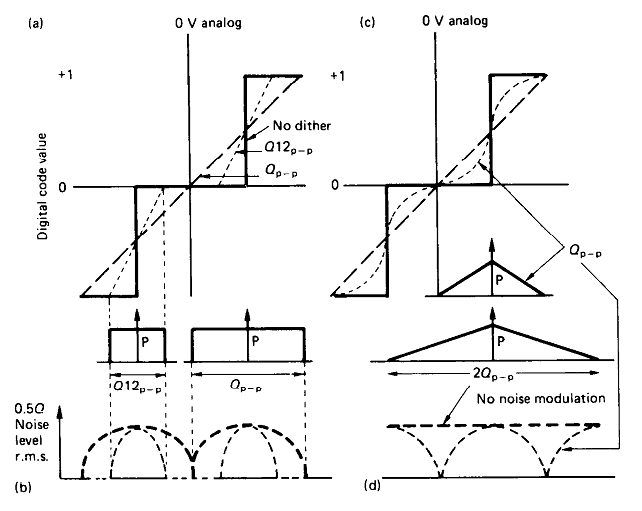
\includegraphics[scale=0.5]{Graph/dither_and_noisemodulation}
			\end{center}
		\end{figure}
	\end{frame}	
	\begin{frame}\frametitle{sampling and quantization}\framesubtitle{requantization and dither: linearization and noise modulation 2/2}
		\begin{figure}
			\begin{center}
					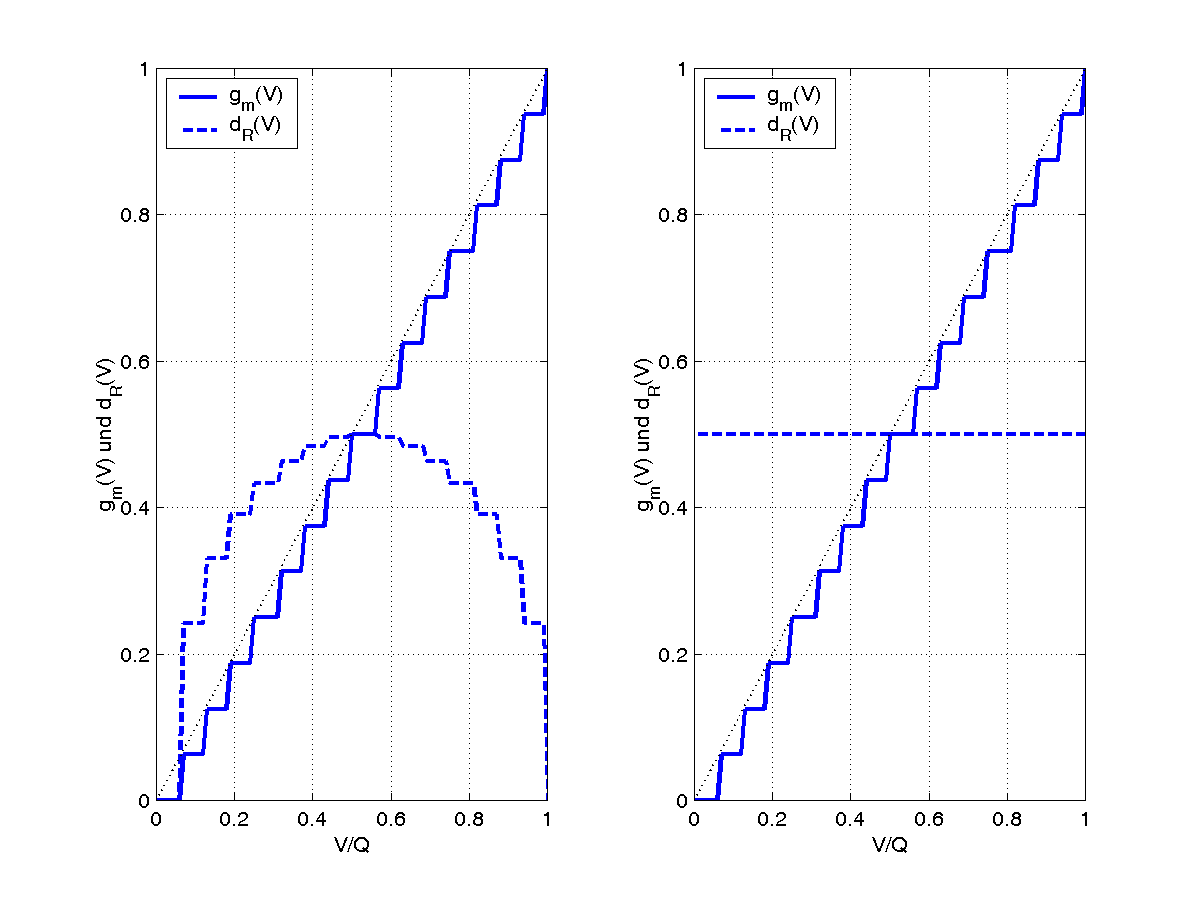
\includegraphics[scale=0.5]{Graph/rauschmodulation}
			\end{center}
		\end{figure}	
	\end{frame}	
	\begin{frame}\frametitle{sampling and quantization}\framesubtitle{requantization and dither: noise properties 1/3}
		\begin{figure}[htbp]
			\centering
				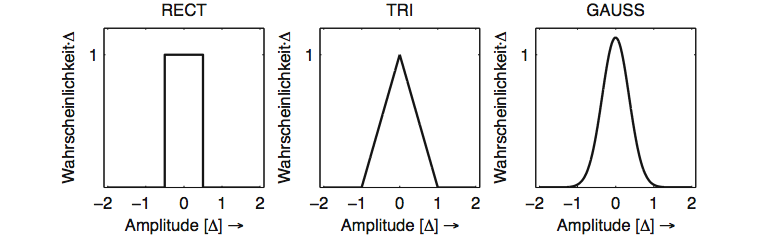
\includegraphics[scale=0.8]{Graph/dither_amplitudendichteverteilung.png}
		\end{figure}
		\pause
		\begin{eqnarray}\label{eq:ditherformen}
			d_\mathrm{RECT}(n) &=& d(n)\\
			d_\mathrm{TRI}(n) &=& d_\mathrm{RECT,1}(n)+d_\mathrm{RECT,2}(n)\\
			\pause
            d_\mathrm{HP}(n) &=& d(n)-d(n-1)
		\end{eqnarray}
	\end{frame}	
	\begin{frame}\frametitle{sampling and quantization}\framesubtitle{requantization and dither: noise properties 2/3}
		\vspace{-3mm}
        \begin{figure}[!hbt]
			\centering
				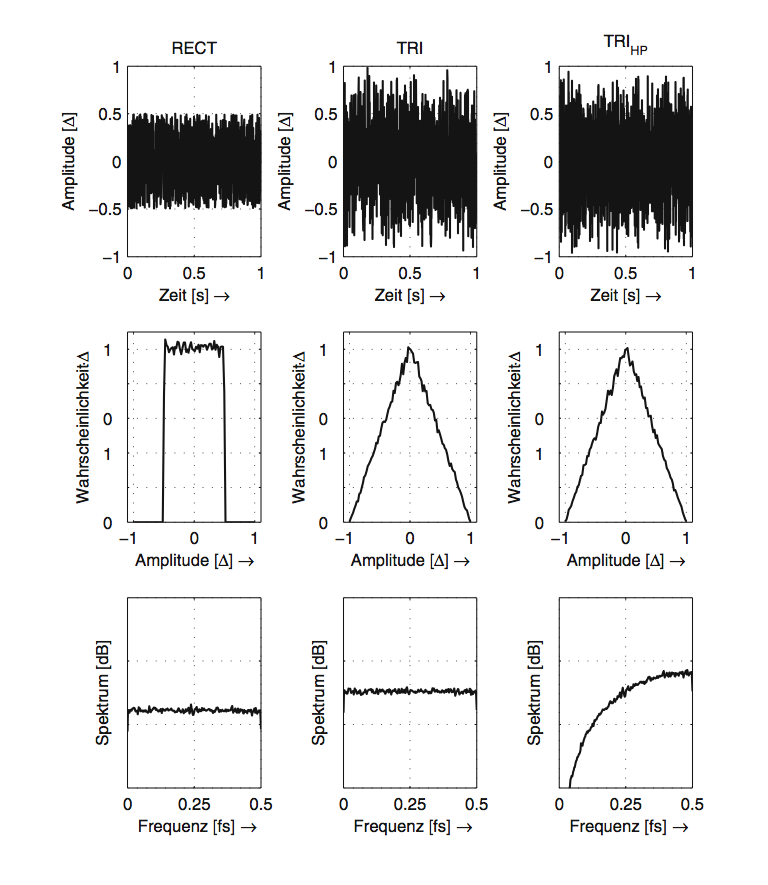
\includegraphics[scale=0.5]{Graph/noiseadv.png}
		\end{figure}
	\end{frame}	
	\begin{frame}\frametitle{sampling and quantization}\framesubtitle{requantization and dither: noise properties 3/3}
		\vspace{-15mm}
		\begin{columns}
			\column{.75\textwidth}
			noise power of $d_{RECT}$ \& $d_{TRI}$
			
			\column{.25\textwidth}
			%\hspace{5mm}
			\begin{flushright}
				 
\includegraphics[scale=.08]{Graph/question-mark}
			\end{flushright}
		\end{columns}
		\pause
		\begin{eqnarray}
			W_{RECT} &=& \frac{\Delta^2}{12}\\
			W_{TRI} &=& \frac{\Delta^2}{6}
		\end{eqnarray}
		\pause
		$\Rightarrow$ SNR of dithered full scale sinusoid:
		\begin{eqnarray}
			SNR_{RECT} 	&= SNR_{normal} - 3.01 &[dB] \\
			SNR_{TRI} 	&= SNR_{normal} - 4.77 &[dB] 
		\end{eqnarray}

	\end{frame}	
	%\begin{frame}\frametitle{sampling and quantization}\framesubtitle{requantization and dither: real world settings}
		%\begin{figure}
			%\centering
				%\includegraphics[scale=1]{Graph/dither_einstellung.png}
		%\end{figure}
	%\end{frame}
	\begin{frame}\frametitle{sampling and quantization}\framesubtitle{requantization and dither: audio examples}
		\begin{itemize}
			\only<1>{
			\item	\textbf{sinusoidal}
                \begin{itemize}
                    \item   \unit[8]{bit}
                        \begin{itemize}
                            \item   truncate: \includeaudio{audio/sine_quant_8bit.mp3}
                            \item   rect: \includeaudio{audio/sine_quant_8bitrect.mp3}
                            \item   tri: \includeaudio{audio/sine_quant_8bittri.mp3}
                        \end{itemize}
                    \item   \unit[4]{bit}
                        \begin{itemize}
                            \item   truncate: \includeaudio{audio/sine_quant_4bit.mp3}
                            \item   rect: \includeaudio{audio/sine_quant_4bitrect.mp3}
                            \item   tri: \includeaudio{audio/sine_quant_4bittri.mp3}
                        \end{itemize}
                    \item   \unit[2]{bit}
                        \begin{itemize}
                            \item   truncate: \includeaudio{audio/sine_quant_2bit.mp3}
                            \item   rect: \includeaudio{audio/sine_quant_2bitrect.mp3}
                            \item   tri: \includeaudio{audio/sine_quant_2bittri.mp3}
                            \item   trihp: \includeaudio{audio/sine_quant_2bittrihp.mp3}
                        \end{itemize}
                \end{itemize}
				}
			\only<2>{
			\item \textbf{speech}
                \begin{itemize}
                    \item   \unit[8]{bit}
                        \begin{itemize}
                            \item   truncate: \includeaudio{audio/sqam_49_female_8bit.mp3}
                            \item   rect: \includeaudio{audio/sqam_49_female_8bitrect.mp3}
                            \item   tri: \includeaudio{audio/sqam_49_female_8bittri.mp3}
                        \end{itemize}
                    \item   \unit[4]{bit}
                        \begin{itemize}
                            \item   truncate: \includeaudio{audio/sqam_49_female_4bit.mp3}
                            \item   rect: \includeaudio{audio/sqam_49_female_4bitrect.mp3}
                            \item   tri: \includeaudio{audio/sqam_49_female_4bittri.mp3}
                        \end{itemize}
                    \item   \unit[2]{bit}
                        \begin{itemize}
                            \item   truncate: \includeaudio{audio/sqam_49_female_2bit.mp3}
                            \item   rect: \includeaudio{audio/sqam_49_female_2bitrect.mp3}
                            \item   tri: \includeaudio{audio/sqam_49_female_2bittri.mp3}
                            \item   trihp: \includeaudio{audio/sqam_49_female_2bittrihp.mp3}
                        \end{itemize}
                \end{itemize}
				}
			\only<3>{
			\item \textbf{music}
                \begin{itemize}
                    \item   \unit[8]{bit}
                        \begin{itemize}
                            \item   truncate: \includeaudio{audio/bigband_8bit.mp3}
                            \item   rect: \includeaudio{audio/bigband_8bitrect.mp3}
                            \item   tri: \includeaudio{audio/bigband_8bittri.mp3}
                        \end{itemize}
                    \item   \unit[4]{bit}
                        \begin{itemize}
                            \item   truncate: \includeaudio{audio/bigband_4bit.mp3}
                            \item   rect: \includeaudio{audio/bigband_4bitrect.mp3}
                            \item   tri: \includeaudio{audio/bigband_4bittri.mp3}
                        \end{itemize}
                    \item   \unit[2]{bit}
                        \begin{itemize}
                            \item   truncate: \includeaudio{audio/bigband_2bit.mp3}
                            \item   rect: \includeaudio{audio/bigband_2bitrect.mp3}
                            \item   tri: \includeaudio{audio/bigband_2bittri.mp3}
                            \item   trihp: \includeaudio{audio/bigband_2bittrihp.mp3}
                        \end{itemize}
                \end{itemize}
				}
		\end{itemize}
	\end{frame}		
